{"payload":{"allShortcutsEnabled":true,"fileTree":{"Reports":{"items":[{"name":"images","path":"Reports/images","contentType":"directory"},{"name":"biblio.bib","path":"Reports/biblio.bib","contentType":"file"},{"name":"james2023evaluating.tex","path":"Reports/james2023evaluating.tex","contentType":"file"},{"name":"liu2014effects.tex","path":"Reports/liu2014effects.tex","contentType":"file"},{"name":"liu2016shared.tex","path":"Reports/liu2016shared.tex","contentType":"file"},{"name":"liu2017coreach.tex","path":"Reports/liu2017coreach.tex","contentType":"file"},{"name":"main.aux","path":"Reports/main.aux","contentType":"file"},{"name":"main.bbl","path":"Reports/main.bbl","contentType":"file"},{"name":"main.bcf","path":"Reports/main.bcf","contentType":"file"},{"name":"main.blg","path":"Reports/main.blg","contentType":"file"},{"name":"main.fdb_latexmk","path":"Reports/main.fdb_latexmk","contentType":"file"},{"name":"main.fls","path":"Reports/main.fls","contentType":"file"},{"name":"main.log","path":"Reports/main.log","contentType":"file"},{"name":"main.out","path":"Reports/main.out","contentType":"file"},{"name":"main.pdf","path":"Reports/main.pdf","contentType":"file"},{"name":"main.run.xml","path":"Reports/main.run.xml","contentType":"file"},{"name":"main.synctex.gz","path":"Reports/main.synctex.gz","contentType":"file"},{"name":"main.tex","path":"Reports/main.tex","contentType":"file"}],"totalCount":18},"":{"items":[{"name":"Code","path":"Code","contentType":"directory"},{"name":"Reports","path":"Reports","contentType":"directory"},{"name":"README.md","path":"README.md","contentType":"file"}],"totalCount":3}},"fileTreeProcessingTime":5.068439,"foldersToFetch":[],"reducedMotionEnabled":"system","repo":{"id":635200149,"defaultBranch":"main","name":"WallVR","ownerLogin":"Jvaljer","currentUserCanPush":true,"isFork":false,"isEmpty":false,"createdAt":"2023-05-02T09:21:24.000+02:00","ownerAvatar":"https://avatars.githubusercontent.com/u/98323161?v=4","public":true,"private":false,"isOrgOwned":false},"symbolsExpanded":true,"treeExpanded":true,"refInfo":{"name":"main","listCacheKey":"v0:1683012368.0","canEdit":true,"refType":"branch","currentOid":"14cb5b0b1de9ca0a9a2423f87b4b6dcdafd63754"},"path":"Reports/liu2017coreach.tex","currentUser":{"id":98323161,"login":"Jvaljer","userEmail":"abbel.haol@gmail.com"},"blob":{"rawLines":["\\subsection*{Effects of Display Size and Navigation Type on a Classification Task}","    \\subparagraph{by : C.Liu, O.Chapuis, M.Beaudouin-Lafon, E.Lecolinet, W.Mackay}","    \\cite{liu2017CoReach}","    \\paragraph{ \\textit{Quick Summary :} ","                \\newline","                \\indent \\indent \\textnormal{This research papers offers a set of Gestures that would allow users of LHRD to interact more","                easily with the contents they wanna manipulate. As the general multi-touch displays are using pretty common ones, these doesn't ","                scale well with a wall-sized display.}","                \\newline","                \\indent \\indent \\textnormal{In this paper, the main worked points are about co-located collaborative navigations, which involves","                more complex dynamics when you're aware of problems like \"gorilla-arm\" or simply the loss of precision for precise manipulation gestures. ","                Also the \\textit{CoReach} set of gestures had to be thought taking care of multiples human factors, such as collaborative strtategies, ","                or even physical constraints.}","                \\newline","                \\indent \\indent \\textnormal{Especially, this research focuses on Collaborative interactions, as most (if not every) of the previous works","                did focus on addressing precision and fatigue problems for single-users. To recap, \\textit{CoReach} focuses on Large Scale Interaction \\& ","                MultiUser Cooperative Actions.} }","    ","    \\paragraph{ \\textit{Motivations :} ","                \\newline","                \\indent \\indent \\textnormal{With the rise of dat-driven decision making, scenarios where people face communication barriers due to domain-specific ","                terms are becomming common place. And as a solution to this problem comes the large interactive spaces, and especially as we're talking about datas ","                visualization and manipulation, LHRDs !} }","","    \\paragraph{\\textit{Gestures:} \\newline}","    \\indent \\indent Obviously, what would be a set of gestures without any gestures ? So here is a scheme showing and explaning the three different","    implemented gestures for the \\textit{CoReach} prototype :","    ","                ","    \\begin{figure}[h]","        \\centering","        \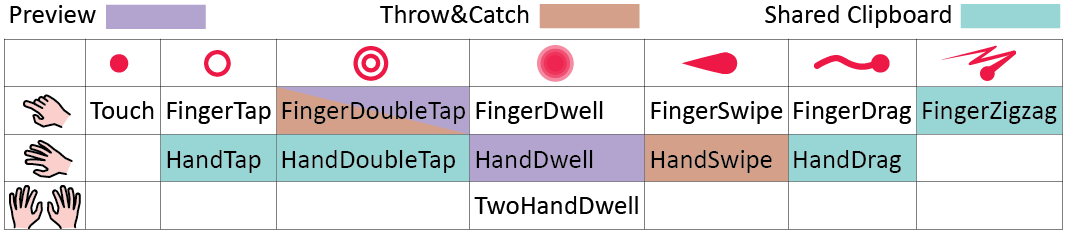
\includegraphics[width=0.5\\textwidth]{images/RecognizedGestures.png}","        \\caption{Figure 1. image taken from the source article (Fig2)}","        \\label{fig:myimage}","    \\end{figure}","    ","    \\indent \\indent So these three recognized gestures were implemented in the prototype, and they're meant to facilitate data-centric","    collaborative tasks on large interactive surfaces. Plus these are especially the pattern gestures that can be applied \\& used by a couple of users in a ","    tasks. Below are detailled these three different gestures and their uses.","","    \\begin{itemize}","        \\item \\textit{Throw and Catch :} This gesture is meant to help people exchange informations by litteraly sending it to each other. It requires a medium level of ","                                        synchronization between the users' actions. ","        \\item \\textit{Preview :} This one is motivated by the fact that users often decides to show their cards to each other, in order to discuss it with more ease. It ","                                requires a high level of synchronization between the users tho. ","        \\item \\textit{Shared Clipboard :} For this last one, it simply provides a way to group items and move them as a whole and not one by one. For some reasons this group is ","                                        temporary (in order to allow the user to rest a bit and ease his use of this feature).","    \\end{itemize}","","    \\paragraph{ \\textit{Study 1 :}","                \\newline}","    \\indent \\indent This first Study is \\textbf{standard vs. Co-Reach Gestures} and has it's titled, is meant to compare a co-located collaboration between two users using standard and co-reach gestures. ","    One of the goals of this is to test the users' acceptance of CoReach gestures. Both contexts are using the same image arrangement, only some instructions were differing between contexts. Also the experiment used ","    logged kinematic to save head movements, users' gestures activations \\& images movements on display. ","    \\newline","    \\indent \\indent And so for the gestures acceptance, results were quite good, as most of participants preferred using Co-Reach gestures instead of standard ones. Plus participants admitted that Co-Reach gestures were ","    funnier to use than the standards. Furthermore the \\textit{Throw \\& Catch} gesture has proved itself as very useful for participant, in addition to be the easiest to learn. ","    \\newline","    \\indent \\indent Finally, as numbered results for this experiment, it made it clear that Co-Reach gestures allowed users to be further from one to another than with the standards. And most used gestures were ","    \\textit{Throw \\& Catch} and \\textit{Preview} as they were far from each others.  ","    ","    \\paragraph{ \\textit{Study 2 :}","                \\newline }","    \\indent \\indent The second Study is \\textbf{Direct vs. Remote Touch} that helped to assess the potential of shared interactions whenever they're at different distance. In other words, the searchers wanted to ","    know in which cases such gestures were the most useful and prefered between direct and remote interactions with/on the wall. TO do that, tablets were  included to the previous experiment, using adapted gestures","    from the Co-Reach ones detailled earlier.","    \\newline ","    \\indent \\indent So in this experiment, some of the gestures are replaced by others (not in their functionment truly, these replacements are more of adaptations than real modifications), plus the context of tasking","    are divided in three, \\textit{Wall Only} (WW), \\textit{Wall+Tablet} (WT), \\textit{Tablet+Tablet} (TT). Which are named explicitely tho. In contrast with the first study, there were less differences to notice between ","    the different contexts. Even tho most participants told that gestures were easier to accept and use direclty on the wall, moreover some of them explained that they felt like working on the wall was making the collaboration","    more natural and logical.","    \\newline","    \\indent \\indent Overall, \\textit{Throw \\& Catch} was still the most used gesture, also, the percentage of use for each gesture was very different from one context to another, in fact being allowed to use a tablet made ","    participants increase their use of \\textit{Share Clipboard}, but made em boo the \\textit{Throw \\& Catch} one.","","    \\paragraph{ \\textit{Discussion :}","                \\newline }","    \\indent \\indent Both studies showed that Co-Reach gestures were nicely adapted to what they were meant for, and so on different aspects ;","    \\begin{itemize}","        \\item First of all it helped to minimize the gesture disruption, because its use was linear (no menu to select or any other mode to switch in between).","        \\item Secondly, the different synchronization levels required by the gestures was very interesting. In fact having a gesture that forces user to be synchronized (at least a little bit) is nice, but here it was even better,","            because users weren't truly forced, as the only gesture which required that level of synchro was one that only requires a \"semi-synchronization\" between users.","        \\item And last but not least, offering a choice between more that one type of gesture allows the users to adapt themselves to the set of gestures. And more precisely it allows people to choose which collaboration strategy","            they're gonna use throughout the experiment.","    \\end{itemize}","    \\indent \\indent But \\textit{Co-Reach} is also an interesting proposition because it doesn't obstructs the users communications, furthermore it made users feel more as a part of a group than as ","    lonely individuals. Which is kinda interesting when it comes to collaborative tasks, but if that so-called group is composed of more than 2 users, then there will be a scalability problem for sure. ","    \\newline","    \\indent \\indent As confirmed in the paper, if there were a third user in the group, the gestures wouldn't be able to suit the tasks as perfeclty as they did for only two users. But perhaps adding other ","    gestures a bit more adapted to a larger group of user could solve this quite easily (as easy asdesigning and implementing such gestures can be tho...). ","","    \\paragraph{ \\textit{Conclusion :}","                \\newline }","    \\indent \\indent As conclusion I've nothing to really add to what I discussed before, the only things to say is that theses gestures has proved to be better than standard ones, but also they seemed","    to been adapted to other uses, like remote uses. And globally, the future possible works would be increasing the possible ways of communication between participants.","    "],"stylingDirectives":[[{"start":0,"end":12,"cssClass":"pl-c1"},{"start":13,"end":81,"cssClass":"pl-en"}],[{"start":4,"end":17,"cssClass":"pl-c1"},{"start":18,"end":81,"cssClass":"pl-en"}],[{"start":4,"end":9,"cssClass":"pl-k"},{"start":10,"end":24,"cssClass":"pl-c1"}],[{"start":4,"end":14,"cssClass":"pl-c1"},{"start":15,"end":41,"cssClass":"pl-en"},{"start":16,"end":23,"cssClass":"pl-c1"},{"start":24,"end":39,"cssClass":"pl-mi"}],[{"start":0,"end":24,"cssClass":"pl-en"},{"start":16,"end":24,"cssClass":"pl-c1"}],[{"start":0,"end":137,"cssClass":"pl-en"},{"start":16,"end":23,"cssClass":"pl-c1"},{"start":24,"end":31,"cssClass":"pl-c1"},{"start":32,"end":43,"cssClass":"pl-c1"}],[{"start":0,"end":144,"cssClass":"pl-en"}],[{"start":0,"end":54,"cssClass":"pl-en"}],[{"start":0,"end":24,"cssClass":"pl-en"},{"start":16,"end":24,"cssClass":"pl-c1"}],[{"start":0,"end":144,"cssClass":"pl-en"},{"start":16,"end":23,"cssClass":"pl-c1"},{"start":24,"end":31,"cssClass":"pl-c1"},{"start":32,"end":43,"cssClass":"pl-c1"}],[{"start":0,"end":154,"cssClass":"pl-en"},{"start":73,"end":86,"cssClass":"pl-ii"}],[{"start":0,"end":151,"cssClass":"pl-en"},{"start":25,"end":32,"cssClass":"pl-c1"},{"start":33,"end":40,"cssClass":"pl-mi"}],[{"start":0,"end":46,"cssClass":"pl-en"}],[{"start":0,"end":24,"cssClass":"pl-en"},{"start":16,"end":24,"cssClass":"pl-c1"}],[{"start":0,"end":153,"cssClass":"pl-en"},{"start":16,"end":23,"cssClass":"pl-c1"},{"start":24,"end":31,"cssClass":"pl-c1"},{"start":32,"end":43,"cssClass":"pl-c1"}],[{"start":0,"end":154,"cssClass":"pl-en"},{"start":99,"end":106,"cssClass":"pl-c1"},{"start":107,"end":114,"cssClass":"pl-mi"},{"start":151,"end":153,"cssClass":"pl-cce"}],[{"start":0,"end":48,"cssClass":"pl-en"}],[],[{"start":4,"end":14,"cssClass":"pl-c1"},{"start":15,"end":39,"cssClass":"pl-en"},{"start":16,"end":23,"cssClass":"pl-c1"},{"start":24,"end":37,"cssClass":"pl-mi"}],[{"start":0,"end":24,"cssClass":"pl-en"},{"start":16,"end":24,"cssClass":"pl-c1"}],[{"start":0,"end":163,"cssClass":"pl-en"},{"start":16,"end":23,"cssClass":"pl-c1"},{"start":24,"end":31,"cssClass":"pl-c1"},{"start":32,"end":43,"cssClass":"pl-c1"}],[{"start":0,"end":164,"cssClass":"pl-en"}],[{"start":0,"end":57,"cssClass":"pl-en"}],[],[{"start":4,"end":14,"cssClass":"pl-c1"},{"start":15,"end":42,"cssClass":"pl-en"},{"start":15,"end":22,"cssClass":"pl-c1"},{"start":23,"end":32,"cssClass":"pl-mi"},{"start":34,"end":42,"cssClass":"pl-c1"}],[{"start":4,"end":11,"cssClass":"pl-c1"},{"start":12,"end":19,"cssClass":"pl-c1"}],[{"start":33,"end":40,"cssClass":"pl-c1"},{"start":41,"end":48,"cssClass":"pl-mi"}],[],[],[{"start":4,"end":10,"cssClass":"pl-c1"},{"start":11,"end":17,"cssClass":"pl-smi"}],[{"start":8,"end":18,"cssClass":"pl-c1"}],[{"start":8,"end":24,"cssClass":"pl-c1"},{"start":34,"end":44,"cssClass":"pl-c1"}],[{"start":8,"end":16,"cssClass":"pl-c1"}],[{"start":8,"end":14,"cssClass":"pl-k"},{"start":15,"end":26,"cssClass":"pl-v"}],[{"start":4,"end":8,"cssClass":"pl-c1"},{"start":9,"end":15,"cssClass":"pl-smi"}],[],[{"start":4,"end":11,"cssClass":"pl-c1"},{"start":12,"end":19,"cssClass":"pl-c1"}],[{"start":122,"end":124,"cssClass":"pl-cce"}],[],[],[{"start":4,"end":10,"cssClass":"pl-c1"},{"start":11,"end":18,"cssClass":"pl-smi"}],[{"start":8,"end":13,"cssClass":"pl-k"},{"start":14,"end":21,"cssClass":"pl-c1"},{"start":22,"end":39,"cssClass":"pl-mi"}],[],[{"start":8,"end":13,"cssClass":"pl-k"},{"start":14,"end":21,"cssClass":"pl-c1"},{"start":22,"end":31,"cssClass":"pl-mi"}],[],[{"start":8,"end":13,"cssClass":"pl-k"},{"start":14,"end":21,"cssClass":"pl-c1"},{"start":22,"end":40,"cssClass":"pl-mi"}],[],[{"start":4,"end":8,"cssClass":"pl-c1"},{"start":9,"end":16,"cssClass":"pl-smi"}],[],[{"start":4,"end":14,"cssClass":"pl-c1"},{"start":15,"end":34,"cssClass":"pl-en"},{"start":16,"end":23,"cssClass":"pl-c1"},{"start":24,"end":33,"cssClass":"pl-mi"}],[{"start":0,"end":24,"cssClass":"pl-en"},{"start":16,"end":24,"cssClass":"pl-c1"}],[{"start":4,"end":11,"cssClass":"pl-c1"},{"start":12,"end":19,"cssClass":"pl-c1"},{"start":40,"end":47,"cssClass":"pl-c1"},{"start":48,"end":78,"cssClass":"pl-mb"}],[],[{"start":73,"end":75,"cssClass":"pl-cce"}],[{"start":4,"end":12,"cssClass":"pl-c1"}],[{"start":4,"end":11,"cssClass":"pl-c1"},{"start":12,"end":19,"cssClass":"pl-c1"}],[{"start":55,"end":62,"cssClass":"pl-c1"},{"start":63,"end":77,"cssClass":"pl-mi"},{"start":69,"end":71,"cssClass":"pl-cce"}],[{"start":4,"end":12,"cssClass":"pl-c1"}],[{"start":4,"end":11,"cssClass":"pl-c1"},{"start":12,"end":19,"cssClass":"pl-c1"}],[{"start":4,"end":11,"cssClass":"pl-c1"},{"start":12,"end":26,"cssClass":"pl-mi"},{"start":18,"end":20,"cssClass":"pl-cce"},{"start":32,"end":39,"cssClass":"pl-c1"},{"start":40,"end":47,"cssClass":"pl-mi"}],[],[{"start":4,"end":14,"cssClass":"pl-c1"},{"start":15,"end":34,"cssClass":"pl-en"},{"start":16,"end":23,"cssClass":"pl-c1"},{"start":24,"end":33,"cssClass":"pl-mi"}],[{"start":0,"end":25,"cssClass":"pl-en"},{"start":16,"end":24,"cssClass":"pl-c1"}],[{"start":4,"end":11,"cssClass":"pl-c1"},{"start":12,"end":19,"cssClass":"pl-c1"},{"start":40,"end":47,"cssClass":"pl-c1"},{"start":48,"end":71,"cssClass":"pl-mb"}],[],[],[{"start":4,"end":12,"cssClass":"pl-c1"}],[{"start":4,"end":11,"cssClass":"pl-c1"},{"start":12,"end":19,"cssClass":"pl-c1"}],[{"start":26,"end":33,"cssClass":"pl-c1"},{"start":34,"end":43,"cssClass":"pl-mi"},{"start":51,"end":58,"cssClass":"pl-c1"},{"start":59,"end":70,"cssClass":"pl-mi"},{"start":78,"end":85,"cssClass":"pl-c1"},{"start":86,"end":99,"cssClass":"pl-mi"}],[],[],[{"start":4,"end":12,"cssClass":"pl-c1"}],[{"start":4,"end":11,"cssClass":"pl-c1"},{"start":12,"end":19,"cssClass":"pl-c1"},{"start":29,"end":36,"cssClass":"pl-c1"},{"start":37,"end":51,"cssClass":"pl-mi"},{"start":43,"end":45,"cssClass":"pl-cce"}],[{"start":39,"end":46,"cssClass":"pl-c1"},{"start":47,"end":62,"cssClass":"pl-mi"},{"start":85,"end":92,"cssClass":"pl-c1"},{"start":93,"end":107,"cssClass":"pl-mi"},{"start":99,"end":101,"cssClass":"pl-cce"}],[],[{"start":4,"end":14,"cssClass":"pl-c1"},{"start":15,"end":37,"cssClass":"pl-en"},{"start":16,"end":23,"cssClass":"pl-c1"},{"start":24,"end":36,"cssClass":"pl-mi"}],[{"start":0,"end":25,"cssClass":"pl-en"},{"start":16,"end":24,"cssClass":"pl-c1"}],[{"start":4,"end":11,"cssClass":"pl-c1"},{"start":12,"end":19,"cssClass":"pl-c1"}],[{"start":4,"end":10,"cssClass":"pl-c1"},{"start":11,"end":18,"cssClass":"pl-smi"}],[{"start":8,"end":13,"cssClass":"pl-k"}],[{"start":8,"end":13,"cssClass":"pl-k"}],[{"start":134,"end":156,"cssClass":"pl-ii"}],[{"start":8,"end":13,"cssClass":"pl-k"}],[],[{"start":4,"end":8,"cssClass":"pl-c1"},{"start":9,"end":16,"cssClass":"pl-smi"}],[{"start":4,"end":11,"cssClass":"pl-c1"},{"start":12,"end":19,"cssClass":"pl-c1"},{"start":24,"end":31,"cssClass":"pl-c1"},{"start":32,"end":40,"cssClass":"pl-mi"}],[],[{"start":4,"end":12,"cssClass":"pl-c1"}],[{"start":4,"end":11,"cssClass":"pl-c1"},{"start":12,"end":19,"cssClass":"pl-c1"}],[],[],[{"start":4,"end":14,"cssClass":"pl-c1"},{"start":15,"end":37,"cssClass":"pl-en"},{"start":16,"end":23,"cssClass":"pl-c1"},{"start":24,"end":36,"cssClass":"pl-mi"}],[{"start":0,"end":25,"cssClass":"pl-en"},{"start":16,"end":24,"cssClass":"pl-c1"}],[{"start":4,"end":11,"cssClass":"pl-c1"},{"start":12,"end":19,"cssClass":"pl-c1"}],[],[]],"csv":null,"csvError":null,"dependabotInfo":{"showConfigurationBanner":null,"configFilePath":null,"networkDependabotPath":"/Jvaljer/WallVR/network/updates","dismissConfigurationNoticePath":"/settings/dismiss-notice/dependabot_configuration_notice","configurationNoticeDismissed":false,"repoAlertsPath":"/Jvaljer/WallVR/security/dependabot","repoSecurityAndAnalysisPath":"/Jvaljer/WallVR/settings/security_analysis","repoOwnerIsOrg":false,"currentUserCanAdminRepo":true},"displayName":"liu2017coreach.tex","displayUrl":"https://github.com/Jvaljer/WallVR/blob/main/Reports/liu2017coreach.tex?raw=true","headerInfo":{"blobSize":"8.73 KB","deleteInfo":{"deleteTooltip":"Delete this file"},"editInfo":{"editTooltip":"Edit this file"},"ghDesktopPath":"x-github-client://openRepo/https://github.com/Jvaljer/WallVR?branch=main&filepath=Reports%2Fliu2017coreach.tex","gitLfsPath":null,"onBranch":true,"shortPath":"ddacfe6","siteNavLoginPath":"/login?return_to=https%3A%2F%2Fgithub.com%2FJvaljer%2FWallVR%2Fblob%2Fmain%2FReports%2Fliu2017coreach.tex","isCSV":false,"isRichtext":false,"toc":null,"lineInfo":{"truncatedLoc":"96","truncatedSloc":"85"},"mode":"file"},"image":false,"isCodeownersFile":null,"isPlain":false,"isValidLegacyIssueTemplate":false,"issueTemplateHelpUrl":"https://docs.github.com/articles/about-issue-and-pull-request-templates","issueTemplate":null,"discussionTemplate":null,"language":"TeX","languageID":369,"large":false,"loggedIn":true,"newDiscussionPath":"/Jvaljer/WallVR/discussions/new","newIssuePath":"/Jvaljer/WallVR/issues/new","planSupportInfo":{"repoIsFork":null,"repoOwnedByCurrentUser":null,"requestFullPath":"/Jvaljer/WallVR/blob/main/Reports/liu2017coreach.tex","showFreeOrgGatedFeatureMessage":null,"showPlanSupportBanner":null,"upgradeDataAttributes":null,"upgradePath":null},"publishBannersInfo":{"dismissActionNoticePath":"/settings/dismiss-notice/publish_action_from_dockerfile","dismissStackNoticePath":"/settings/dismiss-notice/publish_stack_from_file","releasePath":"/Jvaljer/WallVR/releases/new?marketplace=true","showPublishActionBanner":false,"showPublishStackBanner":false},"rawBlobUrl":"https://github.com/Jvaljer/WallVR/raw/main/Reports/liu2017coreach.tex","renderImageOrRaw":false,"richText":null,"renderedFileInfo":null,"shortPath":null,"tabSize":8,"topBannersInfo":{"overridingGlobalFundingFile":false,"globalPreferredFundingPath":null,"repoOwner":"Jvaljer","repoName":"WallVR","showInvalidCitationWarning":false,"citationHelpUrl":"https://docs.github.com/en/github/creating-cloning-and-archiving-repositories/creating-a-repository-on-github/about-citation-files","showDependabotConfigurationBanner":null,"actionsOnboardingTip":null},"truncated":false,"viewable":true,"workflowRedirectUrl":null,"symbols":{"timedOut":false,"notAnalyzed":true,"symbols":[]}},"copilotInfo":{"documentationUrl":"https://docs.github.com/copilot/overview-of-github-copilot/about-github-copilot-for-individuals","notices":{"codeViewPopover":{"dismissed":false,"dismissPath":"/settings/dismiss-notice/code_view_copilot_popover"}},"userAccess":{"accessAllowed":false,"hasSubscriptionEnded":false,"orgHasCFBAccess":false,"userHasCFIAccess":false,"userHasOrgs":false,"userIsOrgAdmin":false,"userIsOrgMember":false,"business":null,"featureRequestInfo":null}},"copilotAccessAllowed":false,"csrf_tokens":{"/Jvaljer/WallVR/branches":{"post":"vcckWEwY7BSSVZeSGxbOvO8H5iAHG4v5RhNrocf7-fpt-AT6nWf75LRTyRfI2SDyWQs6JOTKal8u0tE8IFY2WQ"},"/repos/preferences":{"post":"1EmXX0mTEHiAc7vz62VENFNK5DS0pYTGzb7r3WzJudeYJ8Q-4gCTnGicE3oMIH7D40XSE-IchCVx8Mj782bYtA"}}},"title":"WallVR/Reports/liu2017coreach.tex at main · Jvaljer/WallVR"}